\documentclass[12pt]{article}

\usepackage{amsmath, color}
\usepackage{mdwmath}
\usepackage{amssymb, epsf, epsfig, textcomp}
\renewcommand{\baselinestretch}{1.3}
\usepackage{a4wide}
\newcommand{\argmin}{\mathop{\mathrm{argmin}}}
\usepackage{caption}
\usepackage{subcaption}
\usepackage{mathtools}
\usepackage{listings}
\lstdefinestyle{myCustomMatlabStyle}{
	basicstyle=\ttfamily\footnotesize,
	breaklines=true,
	language=Matlab,
	numbers=left,
	stepnumber=1,
	numbersep=10pt,
	tabsize=4,
	showspaces=false,
	showstringspaces=false
}
\begin{document}
	\noindent\rule{\textwidth}{2pt}
	\begin{center}
		{\bf Technical University of Crete}\\
		{\bf School of Electrical and Computer Engineering} \\
		Course: {\bf Wireless Communications 2022-2023} \\
		Exercise 3 \\%(120/1000) \\
		Report Delivery Date: 8 December 2022 \\
		Instructor: Athanasios P. Liavas \\
	\end{center}
	{\bf Student: }Alevrakis Dimitrios 2017030001\\
	\rule{\textwidth}{.5pt}
	\vskip .1cm
	\noindent
	
	\begin{enumerate}
		\item[Part 1]
			Study of DS-CDMA. Assume communication with $M$-length packets of dual same-probability symbols from the alphabet $\mathcal{X}=\{+1,-1\}$\\
			Every user uses $N$-length code with white gaussian noise characteristics.\\
			Each User utilizes an $L$-length complex impulse response. he response is the same for each packet and changes from packet ot packet.
			\begin{lstlisting}[language=octave]
K = 1; % User Number
M = 300; % Sequence lengh
N = 64; % Code Length
L = 3; % Responce Length
Packets = 1000;
X = [1, -1];

%User code
c = (1/sqrt(N))*sign(randn(N,K));

%Channel response
h = (randn(K,L) + 1i*randn(K,L))*sqrt(1/(2*L));
			\end{lstlisting}
		
			We are decoding the fist user with a Rake receiver (the same process is utilized for the other users).
			
			\begin{enumerate}
				\item One user in the system
				\begin{enumerate}
					\item By concentrating on the decision for the first symbol ($s_1$): The system input is described by the following equality:
					\begin{align*}
						{\bf y} = \sum_{l=1}^{L}h_l{\bf x}^{(l)} + {\bf w}
					\end{align*}
					Where ${\bf x}^(l)=s_1{\bf c}^{(l)}$\\
					and
					\begin{align*}
						{\bf c}^{(l)}\coloneq \begin{bmatrix}
							{\bf 0}_l \\ {\bf c} \\ {\bf 0}_{L-l} 
						\end{bmatrix}
					\end{align*}
				
					Assuming that $||{\bf c}^{(l)}||=1$ and ${\bf c}^(l)^T{\bf c}^{(m)}=0$.
					
					Then the $i-th$ finger output for $i=1,...,L$ is
					\begin{align*}
						\frac{|h_i|^2}{||{\bf h}||}s+w'_i
					\end{align*}
					Where $\displaystyle w'_i\sim \mathcal{CN}(0,\frac{|h_i|^2}{||{\bf h}||^2}N_0)$
					
					and the Rake output is:
					\begin{align*}
						r = ||{\bf h}||s+w'',\ w''\sim\mathcal{CN}(0,N_0)
					\end{align*}
				
					\begin{figure}[h!]
						\centering
						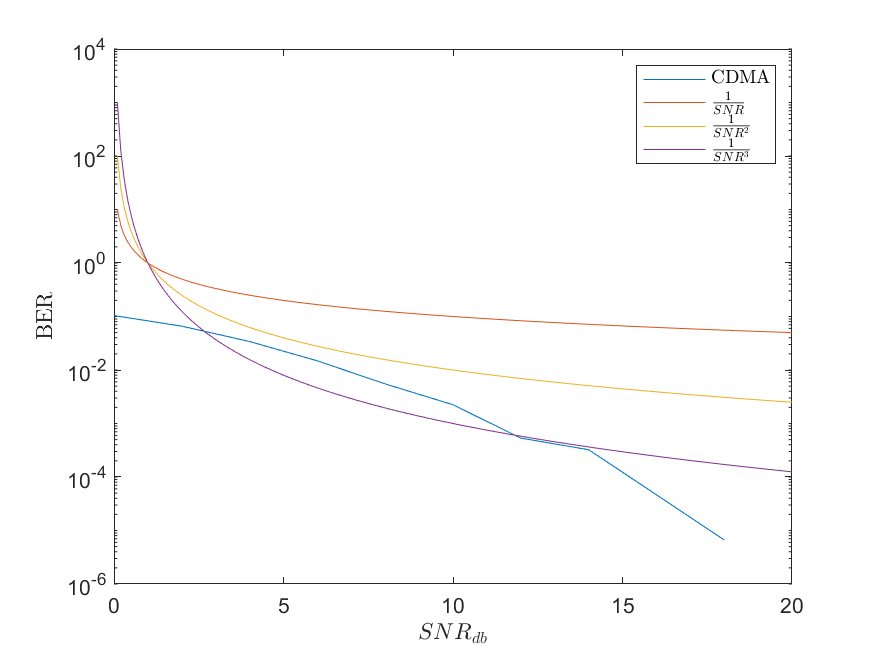
\includegraphics[width=0.5\textwidth]{fig1.png}
						\caption{CDMA comparison with $\frac{1}{SNR^i}$ and one user}
					\end{figure}
				
					\item The Rake receiver using only the highest amplitude channel factor
					\begin{figure}[h!]
						\centering
						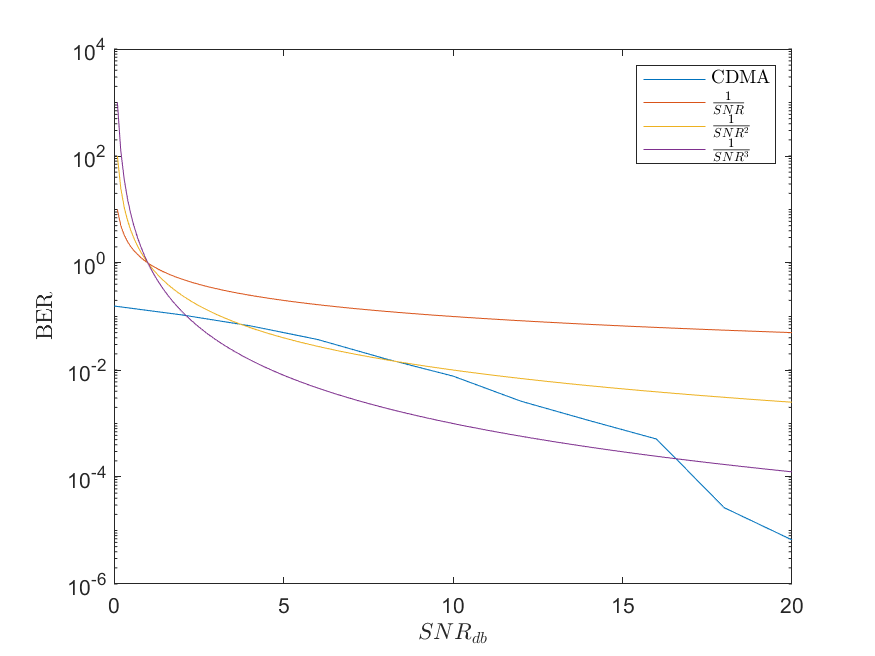
\includegraphics[width=0.5\textwidth]{fig2.png}
						\caption{CDMA comparison with $\frac{1}{SNR^i}$ and one user using stronger channel factor}
					\end{figure}
				
					For low SNRs the Rake receiver with one finger achieves order 2 diversity and for high SNRs order 3. While with L fingers the diversity order is always 3.\\
				
					Compared to using all the channel factor the performance is comparable but in the highest SNRs using all channel factor achieves the lowest BER. 
					\end{enumerate}
					
					\newpage
					\item Multiple users in the system
					\begin{enumerate}
						\item Two Users
							\begin{figure}[h!]
								\centering
								\begin{subfigure}[b]{0.4\textwidth}
									\centering
									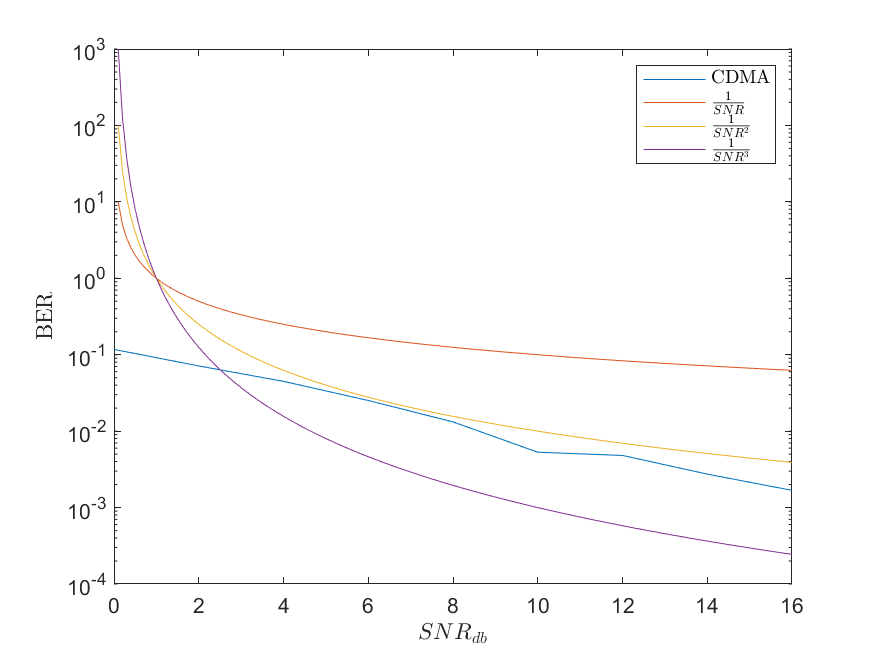
\includegraphics[width=0.9\textwidth]{fig3.png}
									\caption{N=16}
								\end{subfigure}
								\begin{subfigure}[b]{0.4\textwidth}
									\centering
									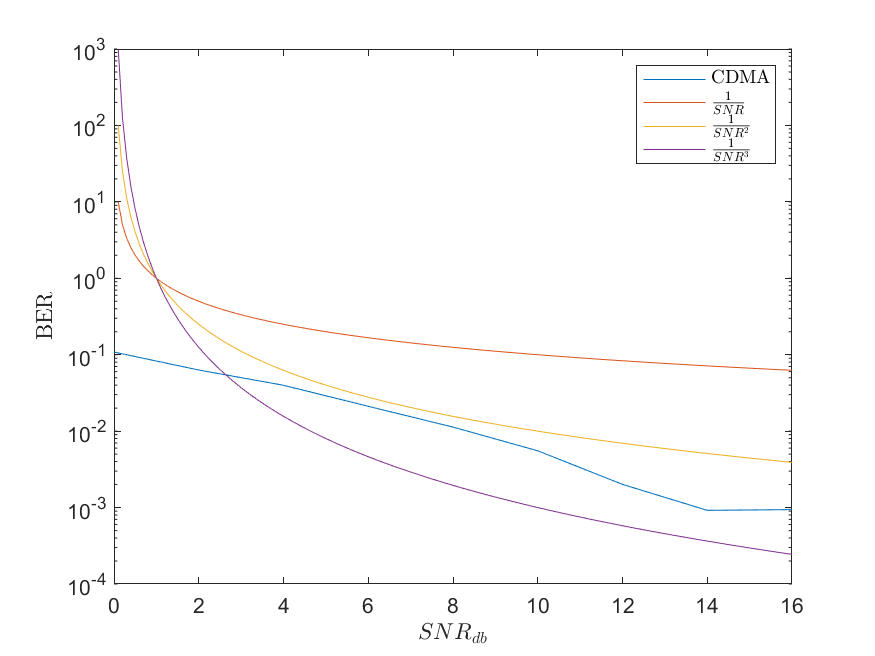
\includegraphics[width=0.9\textwidth]{fig4.png}
									\caption{N=32}
								\end{subfigure}
								\begin{subfigure}[b]{0.4\textwidth}
									\centering
									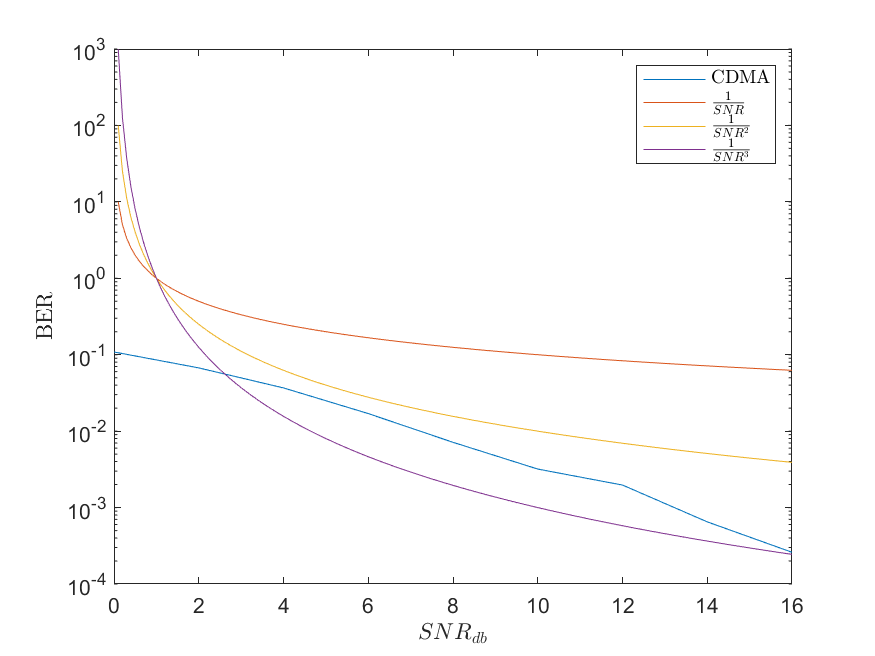
\includegraphics[width=0.9\textwidth]{fig5.png}
									\caption{N=64}
								\end{subfigure}
								\begin{subfigure}[b]{0.4\textwidth}
									\centering
									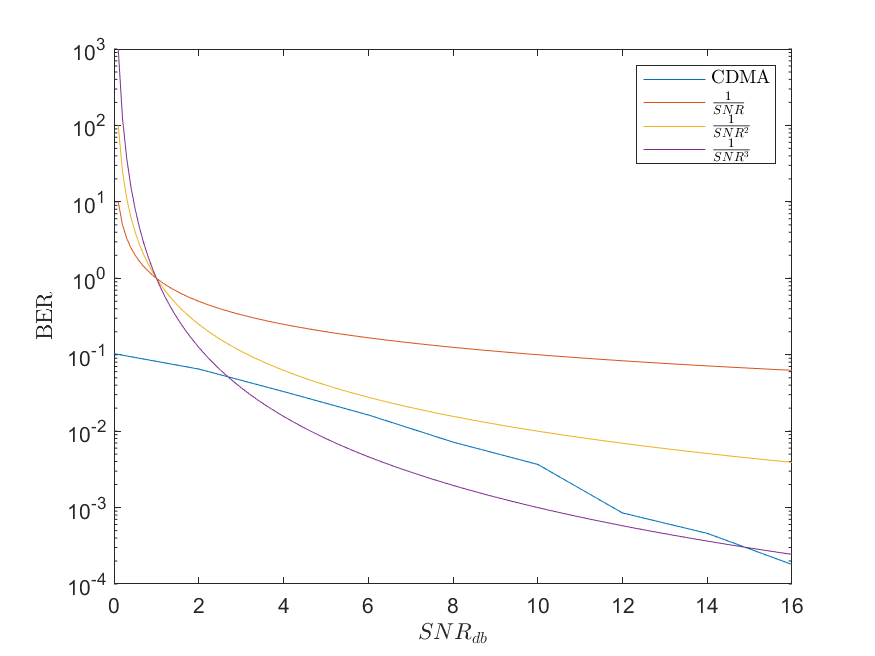
\includegraphics[width=0.9\textwidth]{fig6.png}
									\caption{N=128}
								\end{subfigure}
								\caption{CDMA comparison with $\frac{1}{SNR^i}$ and two users}
							\end{figure}
						
							As seen from Figure 3 when $N=16$ the Rake receiver achieves order 2 diversity and as $N$ goes to $N=128$ it achieves order 3 diversity.
							
							\newpage
							\item Five Users
							\begin{figure}[h!]
								\centering
								\begin{subfigure}[b]{0.4\textwidth}
									\centering
									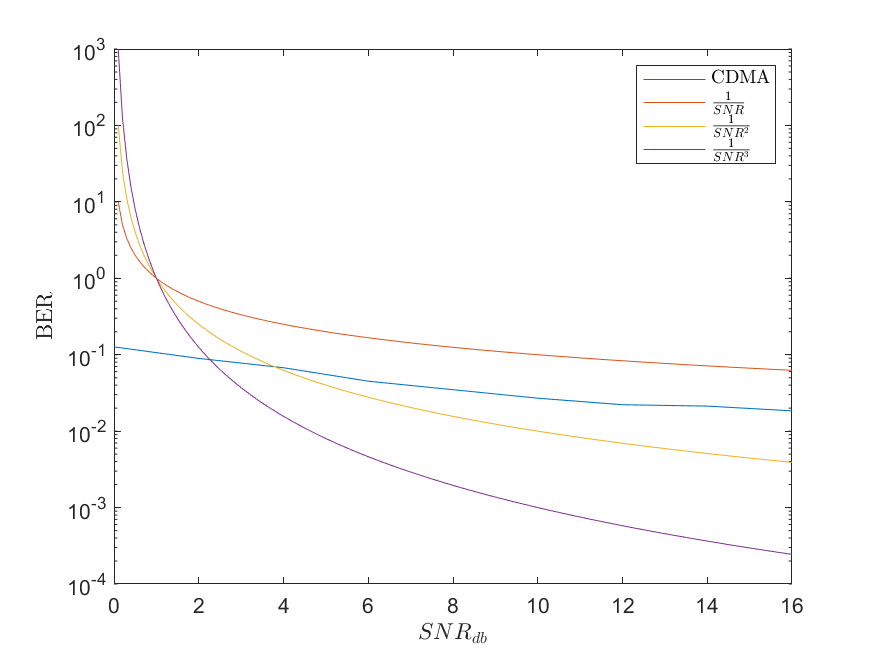
\includegraphics[width=0.9\textwidth]{fig7.png}
									\caption{N=16}
								\end{subfigure}
								\begin{subfigure}[b]{0.4\textwidth}
									\centering
									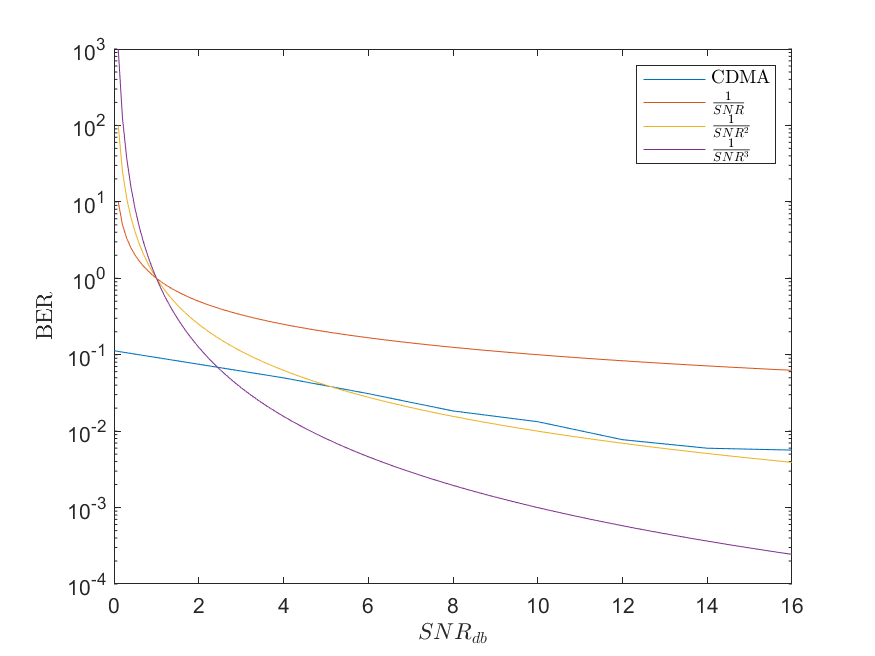
\includegraphics[width=0.9\textwidth]{fig8.png}
									\caption{N=32}
								\end{subfigure}
								\begin{subfigure}[b]{0.4\textwidth}
									\centering
									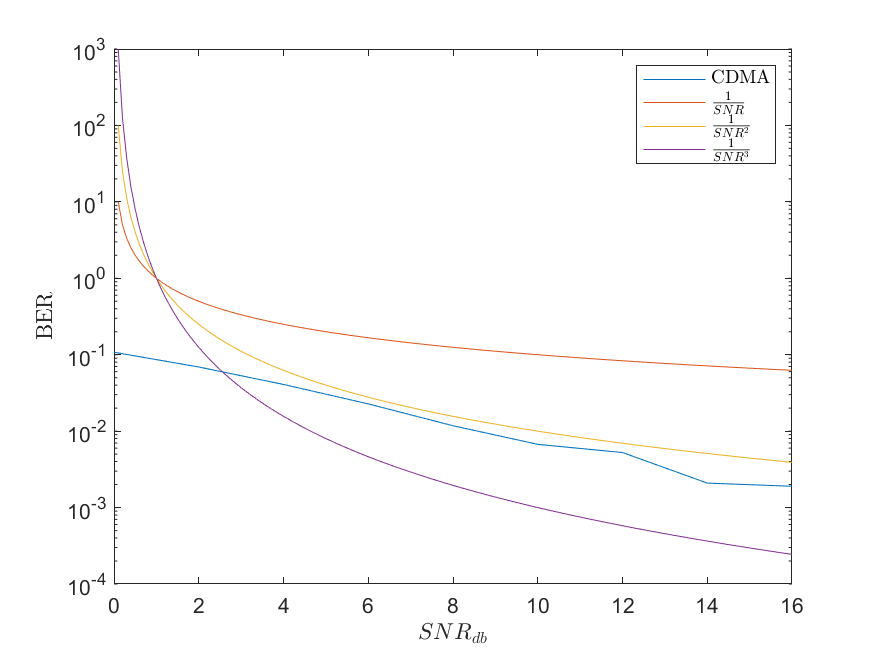
\includegraphics[width=0.9\textwidth]{fig9.png}
									\caption{N=64}
								\end{subfigure}
								\begin{subfigure}[b]{0.4\textwidth}
									\centering
									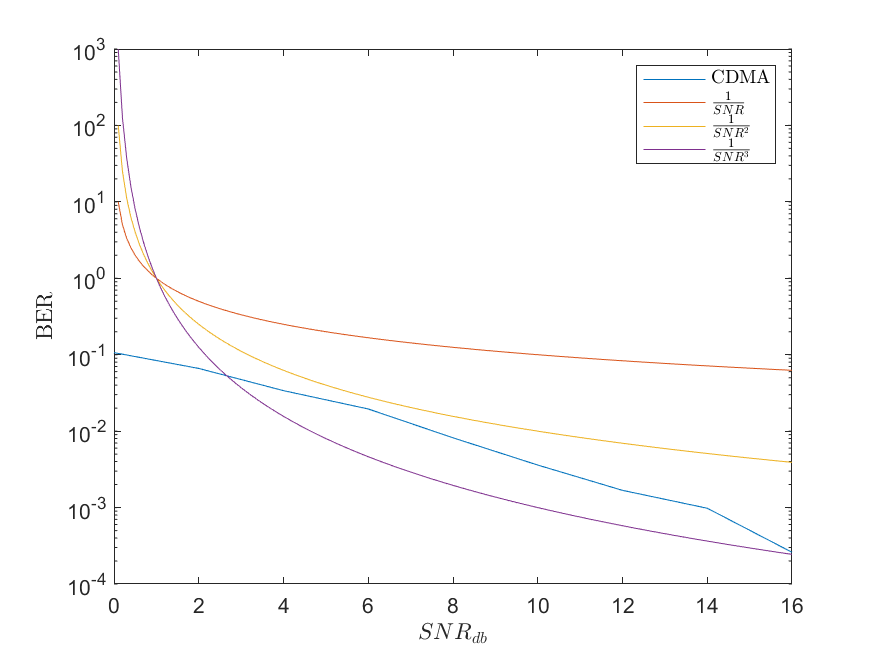
\includegraphics[width=0.9\textwidth]{fig10.png}
									\caption{N=128}
								\end{subfigure}
								\caption{CDMA comparison with $\frac{1}{SNR^i}$ and five users}
							\end{figure}
						
							In the case of five users the performance seems to also achieve better diversity a $N$ increases but for low $N$ the BER does not decreace significantly as SNR increases. 
					\end{enumerate}
			\end{enumerate}
		
		\item[Part 2]
		\begin{enumerate}
			\item 
				\begin{enumerate}
					\item Creation of a random complex channel $h_l$, $l=,0,..,L$ where $h_i$ i.i.d $h_i \sim \mathcal{CN}(0,\frac{1}{L})$
					\begin{lstlisting}[language=octave]
% Channel response
h = (randn(L,1) + 1i*randn(L,1))*sqrt(1/(2*L));
					\end{lstlisting}
				
					\item Creation of 4-QAM input $\tilde{d}$, $k=1,...N$ with values $\pm 1 \pm j$
					
					\begin{lstlisting}[language=octave]
% 4-QAM data block
d = sign(-1+2*rand(N,1)) + 1i*sign(-1+2*rand(N,1));
d_tilde = (1/sqrt(N))*fft(d,N);
					\end{lstlisting}
				
					\item In order to be convinced that the frequency selective channel is equal to N parallel channels the two equalities mast produce the same output.
					
					Equality 1:
					\begin{align*}
						y[m] = \sum_{l=0}^{L-1}h_lx[m-l], m=1,...,N+L-1
					\end{align*} 
					
					Where,
					\begin{align*}
						{\bf x} = \begin{bmatrix}
							d[N-L+2] \\ \vdots \\ d[N] \\ d[1] \\ \vdots \\ d[N]
						\end{bmatrix}
					\end{align*}
				
					Ignoring the first $L-1$ elements we get $y'$ the channel output.
					
					Equality 2:
					\begin{align*}
						\tilde{y} = \tilde{h}\tilde{d}
					\end{align*}
					Where 
					\begin{align*}
						\tilde{h} = DFT(h)\\
						\tilde{d} = DFT(d)
					\end{align*}
				
					In order for the claim to be true then it must be true that:
					\begin{align*}
						y' = IDFT(\tilde{y})
					\end{align*}
					
					\begin{figure}[h!]
						\centering
						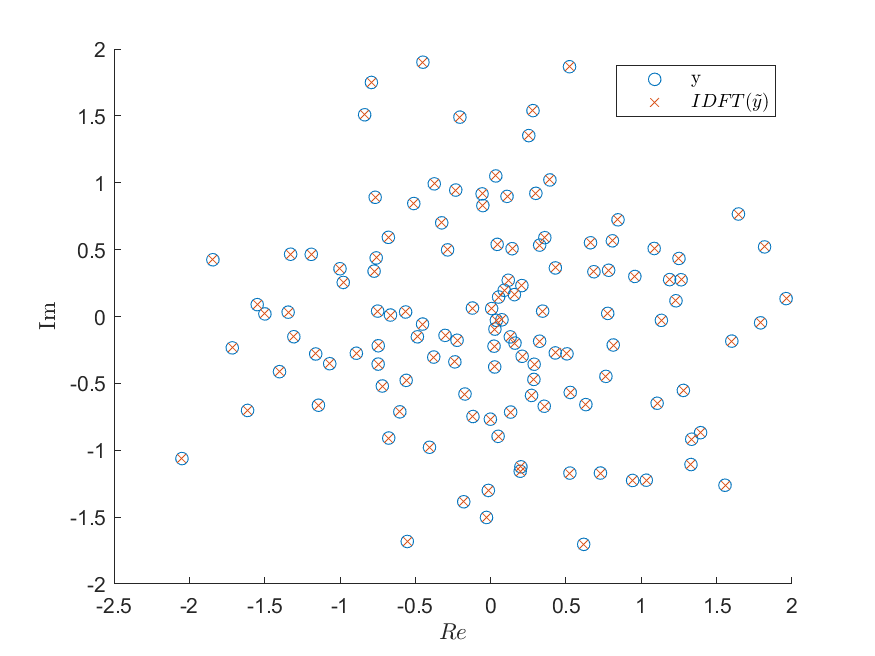
\includegraphics[width=0.5\textwidth]{fig11.png}
						\caption{Frequency Selective to N-Parallel channel output comparison}
					\end{figure}
				
					\newpage
					\item 
					\begin{figure}[h!]
						\centering
						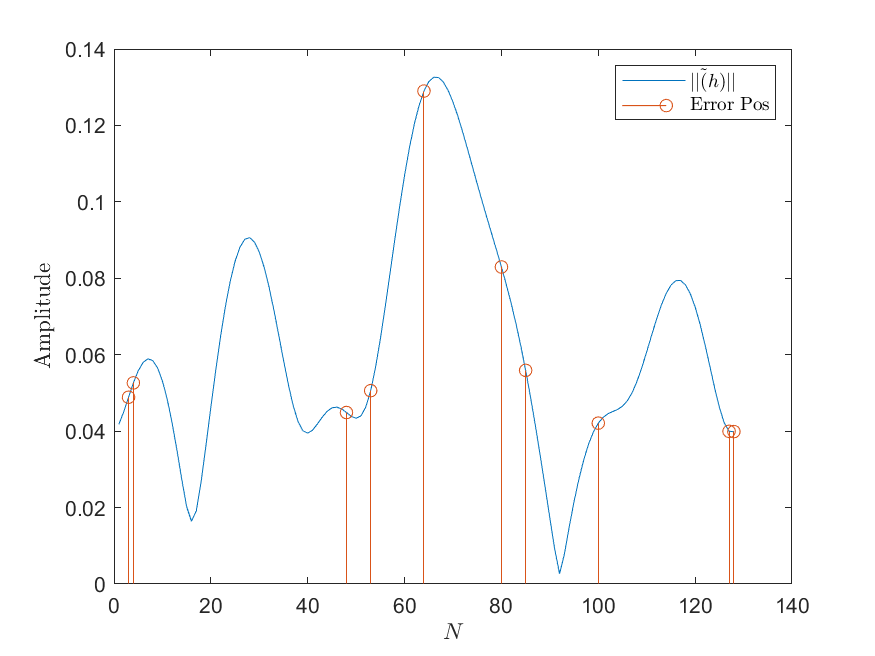
\includegraphics[width=0.5\textwidth]{fig12.png}
						\caption{Channel Amplitude compared to decision error}
					\end{figure}
					There is no obvious correlation to the channel response  amplitude and when the mistakes happen.
				\end{enumerate}
			
					
			\item
			
		\end{enumerate}
	\end{enumerate}
	
\end{document}
